\chapter{determination of exchange stiffnessness}



\section{Measurement of ST-FMR on circular devices}


\begin{figure}[!ht]
\centering
\subfigure{\label{fig:C07MR}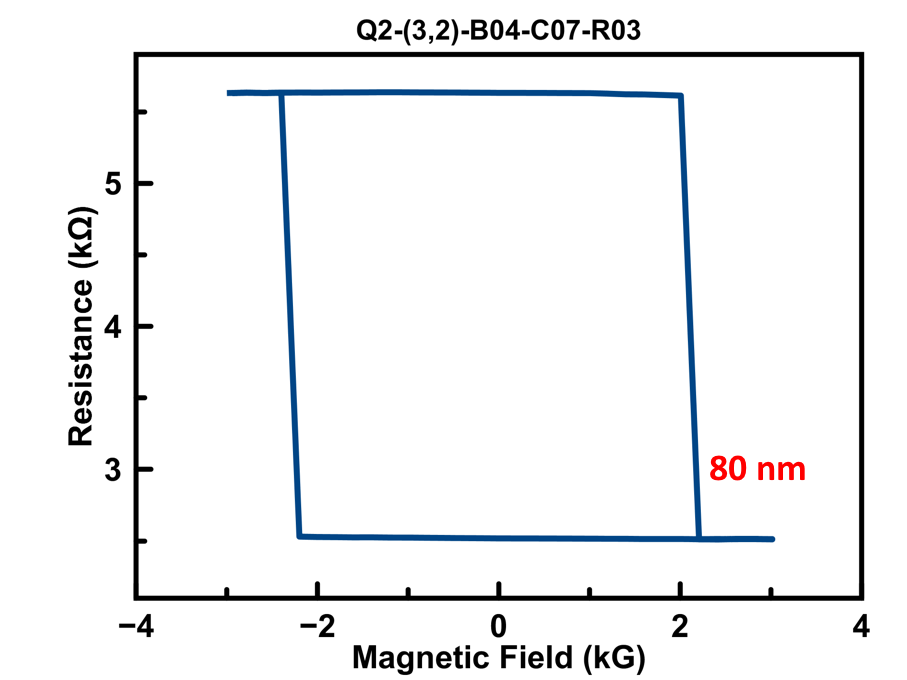
\includegraphics[width=75mm]{fig/2018/C07MR}}
\subfigure{\label{fig:C07FH}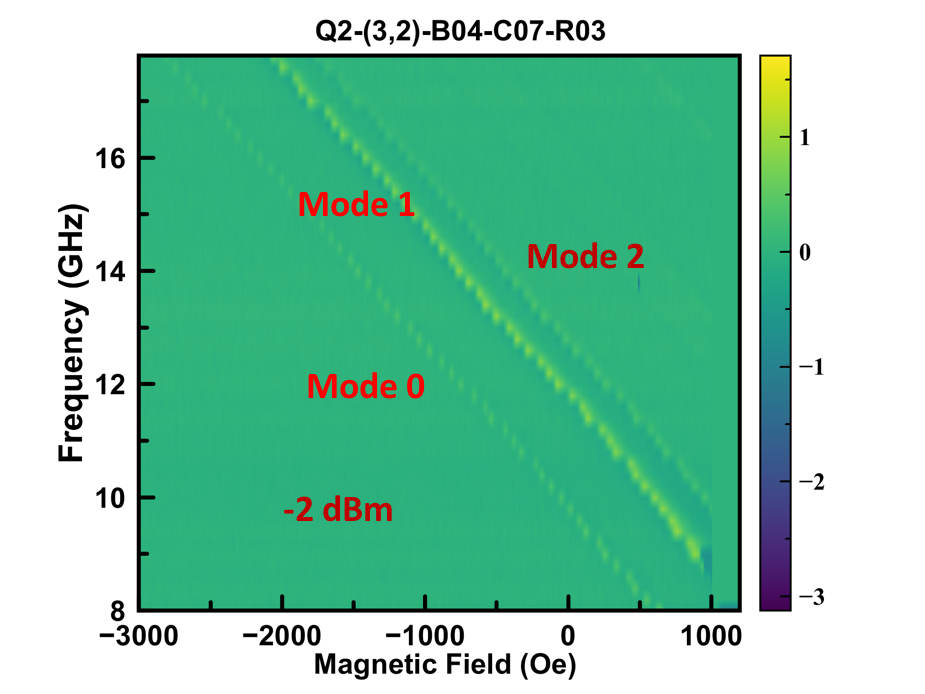
\includegraphics[width=75mm]{fig/2018/C07FH}}
\caption{}
\end{figure}




\begin{figure}[!ht]
  \centering
  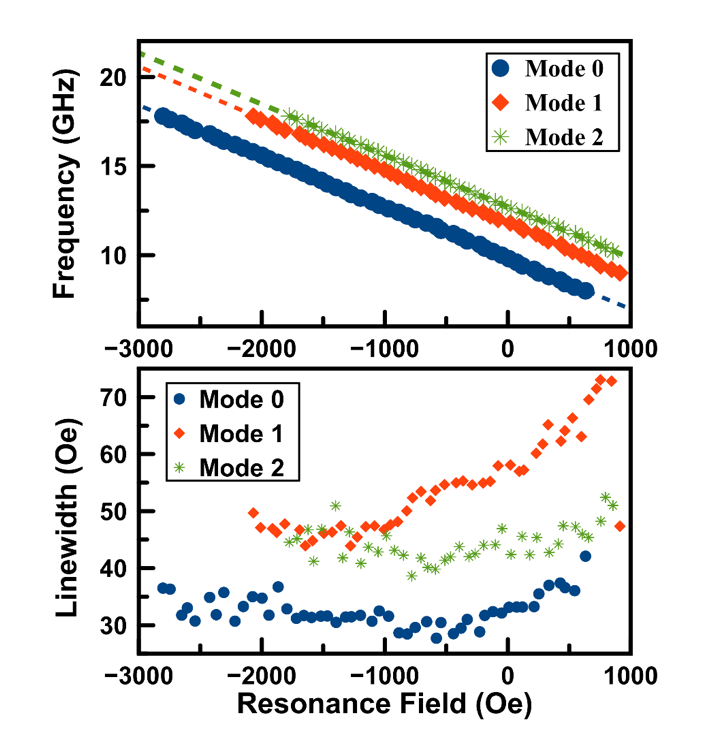
\includegraphics[width=0.6\textwidth]{fig/2018/C07fit}
   \caption{07 sample fit}
  \label{fig:07fit}
\end{figure}





\newpage



\section{Study of signal amplitude of ST-FMR signal}


\begin{figure}[!ht]
\centering
\subfigure{\label{fig:C10MR}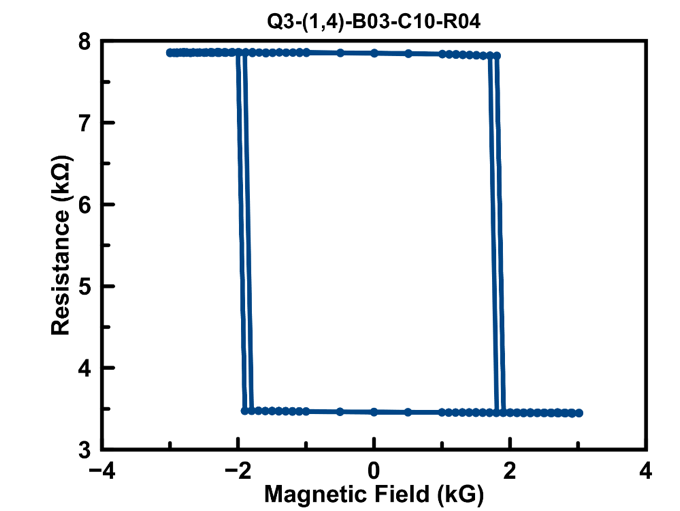
\includegraphics[width=50mm]{fig/2018/C10MR}}
\subfigure{\label{fig:C10RDC}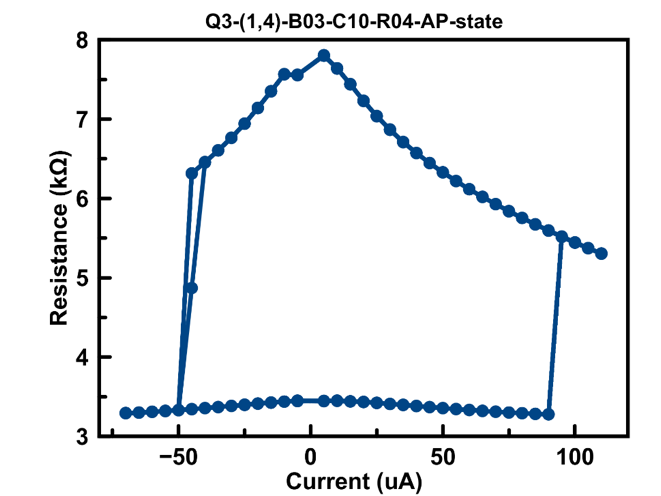
\includegraphics[width=50mm]{fig/2018/C10RDC}}
\subfigure{\label{fig:C102D}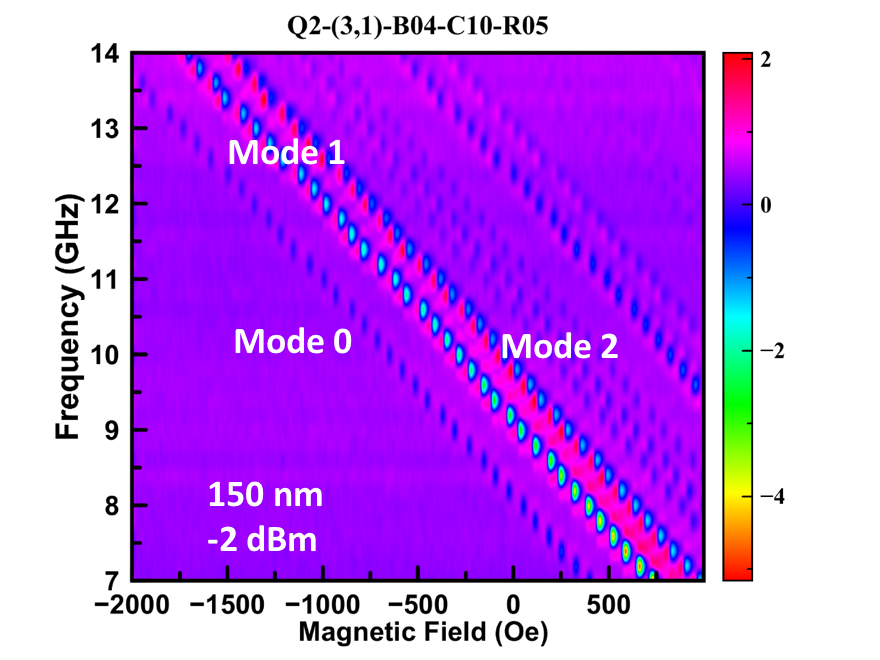
\includegraphics[width=50mm]{fig/2018/C102D}}
\caption{}
\end{figure}



\begin{figure}[!ht]
\centering
\subfigure{\label{fig:C10FH}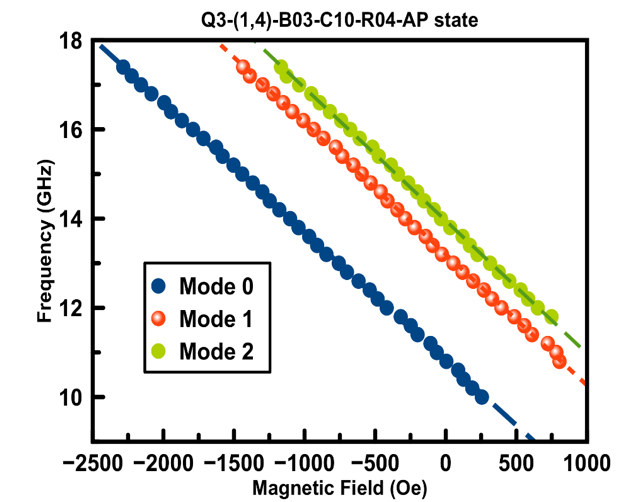
\includegraphics[width=50mm]{fig/2018/C10fit}}
\subfigure{\label{fig:C10signal}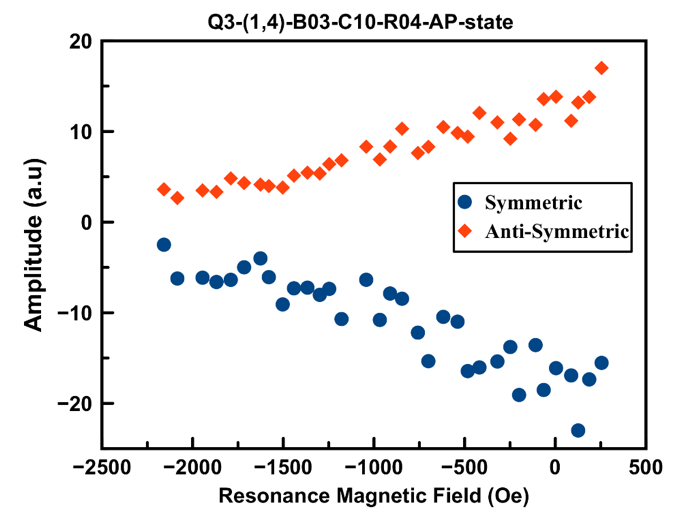
\includegraphics[width=50mm]{fig/2018/C10signal}}
\subfigure{\label{fig:C10ratio}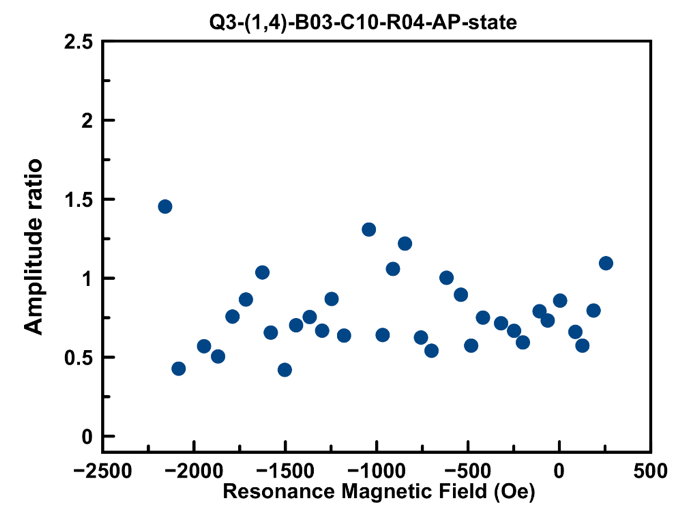
\includegraphics[width=50mm]{fig/2018/C10ratio}}
\caption{}
\end{figure}




\begin{figure}[!ht]
\centering
\subfigure{\label{fig:C10power}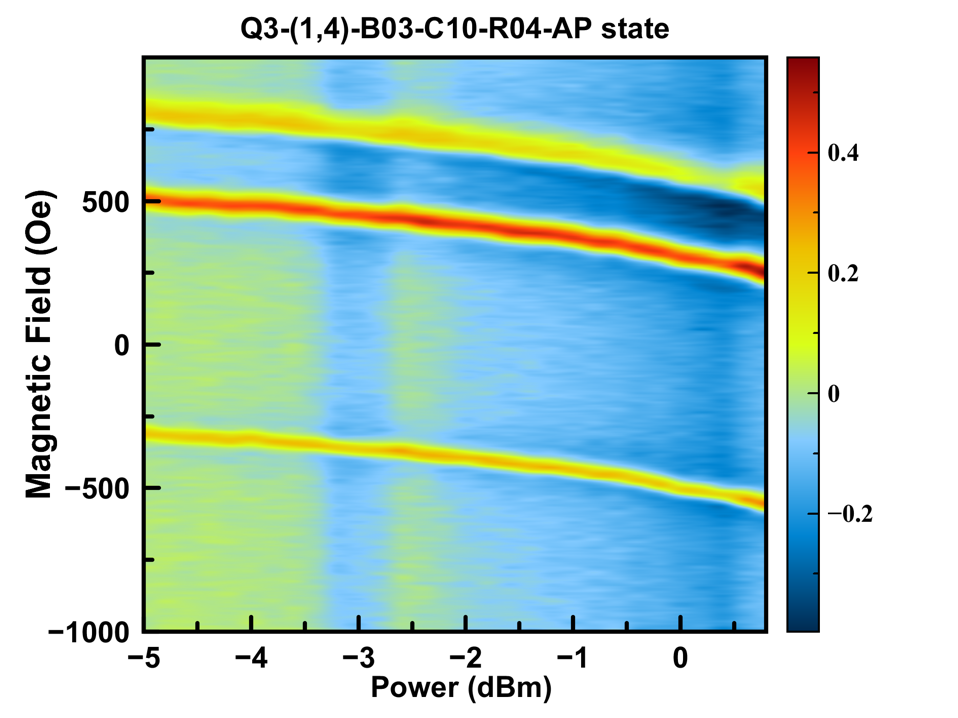
\includegraphics[width=75mm]{fig/2018/C10power}}
\subfigure{\label{fig:C10poweramp}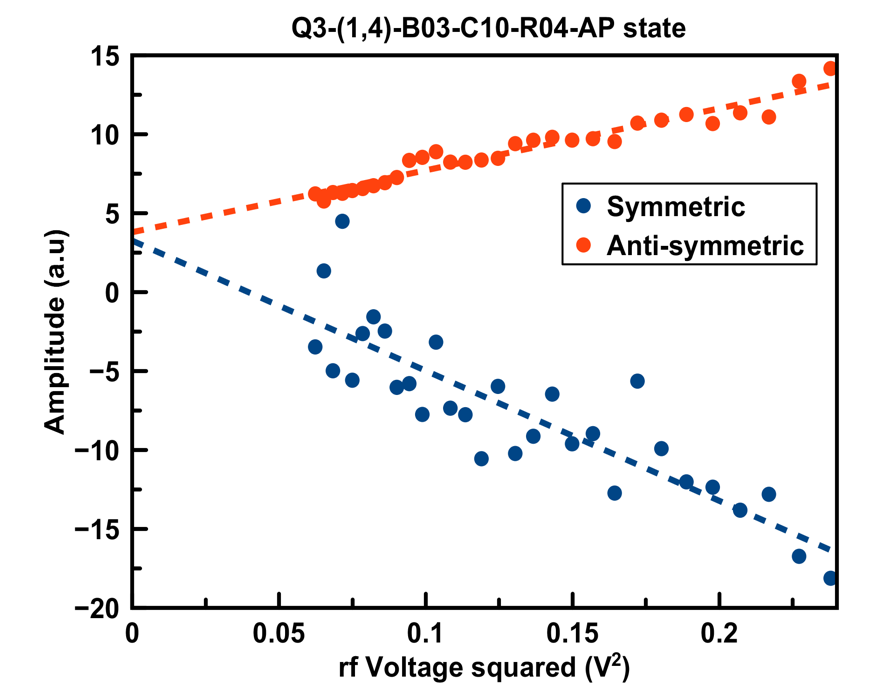
\includegraphics[width=75mm]{fig/2018/C10powersignal}}
\caption{}
\end{figure}




\begin{figure}[!ht]
\centering
\subfigure{\label{fig:C10powerfit}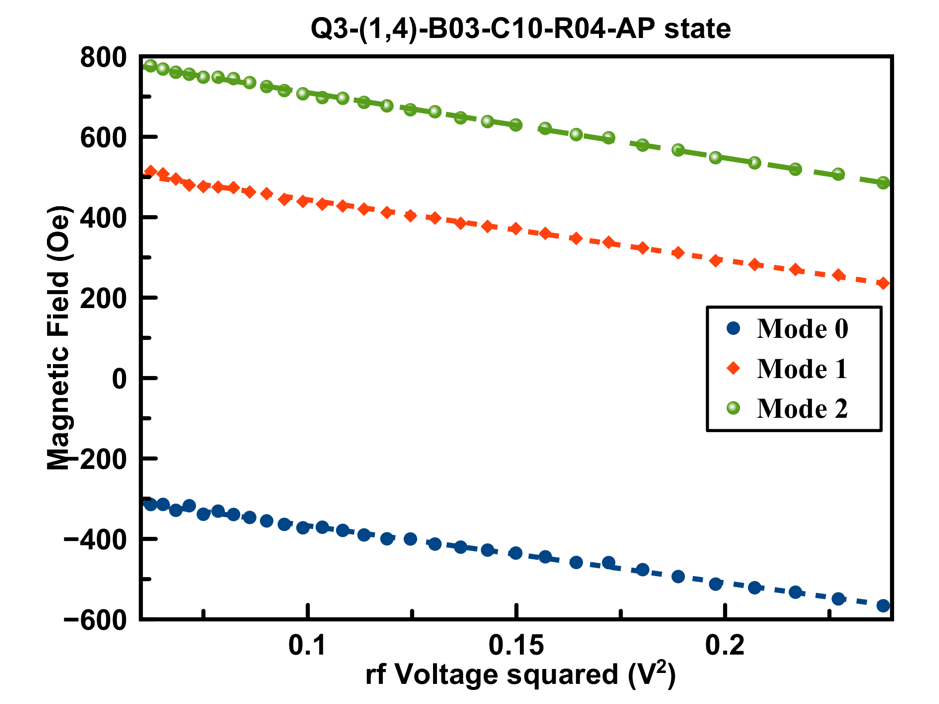
\includegraphics[width=75mm]{fig/2018/C10powerFH}}
\subfigure{\label{fig:C10powerLW}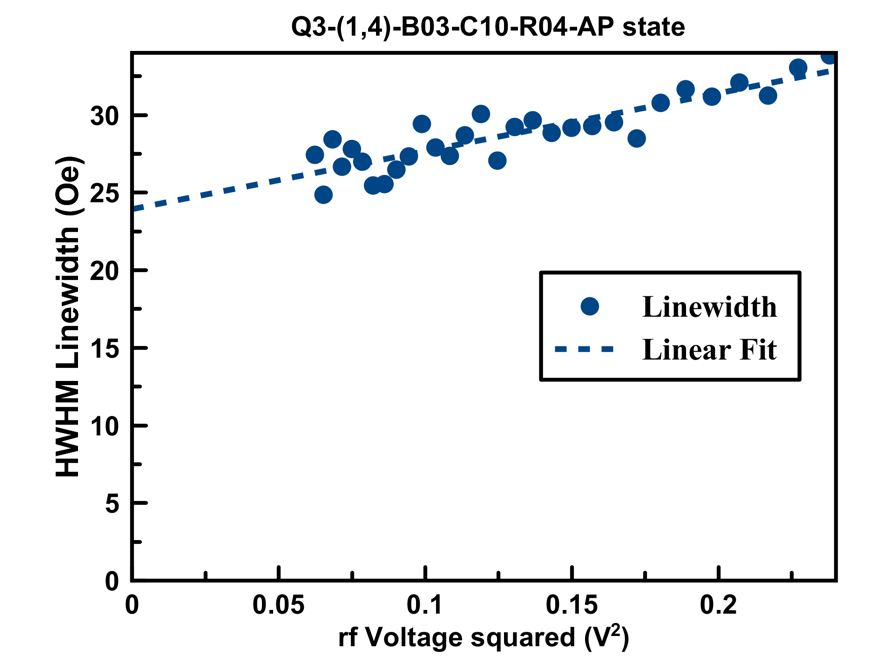
\includegraphics[width=75mm]{fig/2018/C10powerLW}}
\caption{}
\end{figure}

\begin{figure}[!ht]
\centering
\subfigure{\label{fig:C10DC}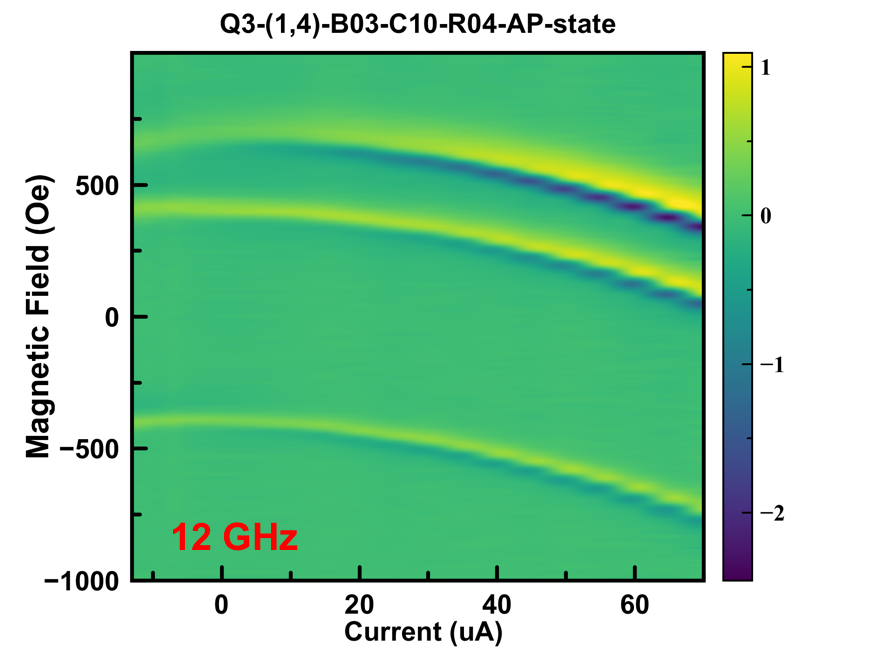
\includegraphics[width=75mm]{fig/2018/C10DC}}
\subfigure{\label{fig:C10DCamp}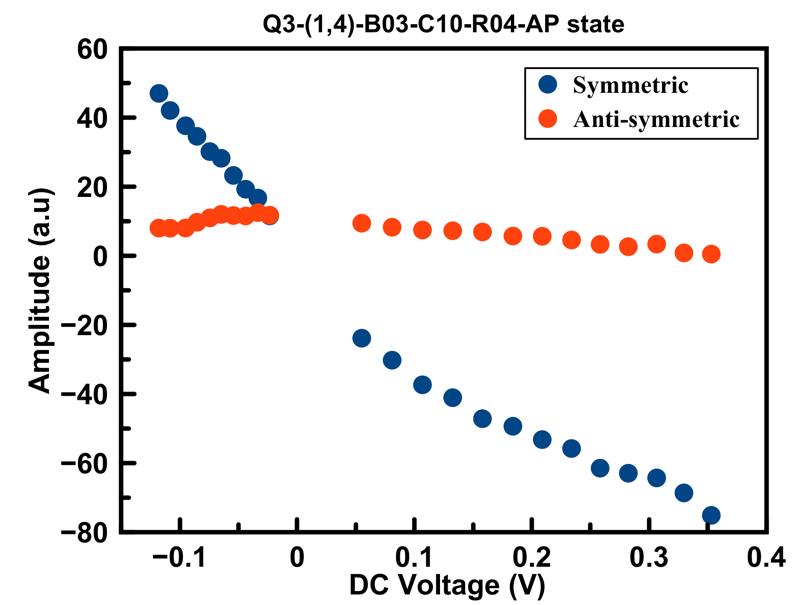
\includegraphics[width=75mm]{fig/2018/C10DCsignal}}
\caption{}
\end{figure}




\begin{figure}[!ht]
  \centering
  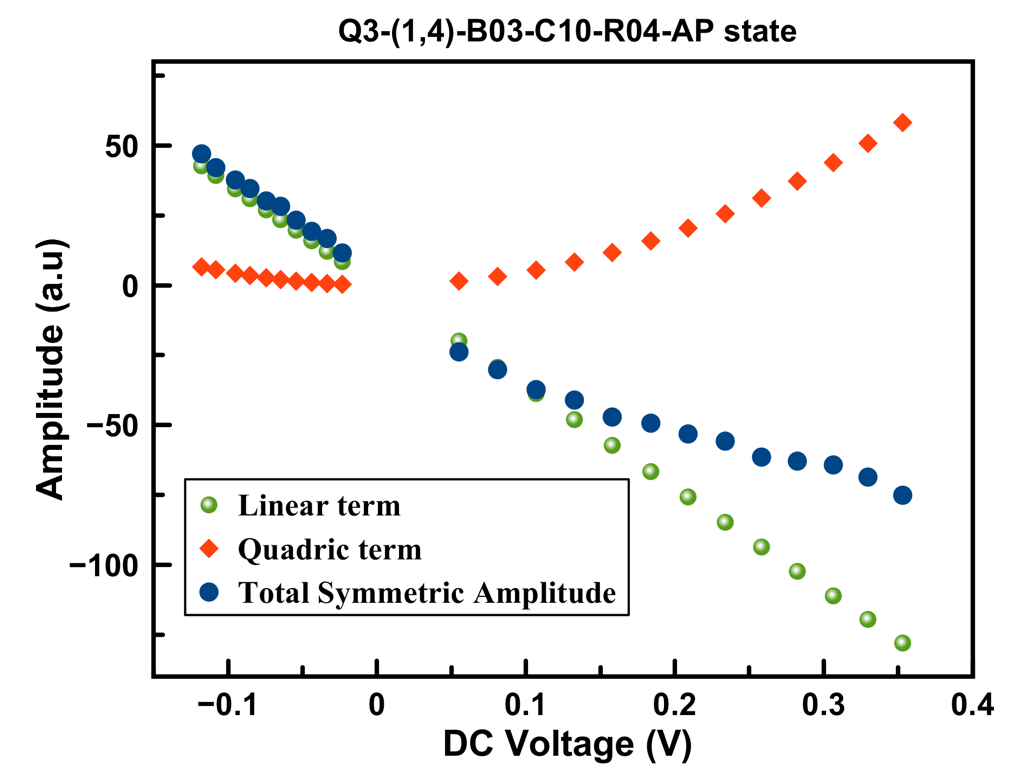
\includegraphics[width=0.8\textwidth]{fig/2018/C10DCFIT}
   \caption{C10 sample fit}
  \label{fig:C10DCfit}
\end{figure}



\begin{figure}[!ht]
\centering
\subfigure{\label{fig:C10DCFH}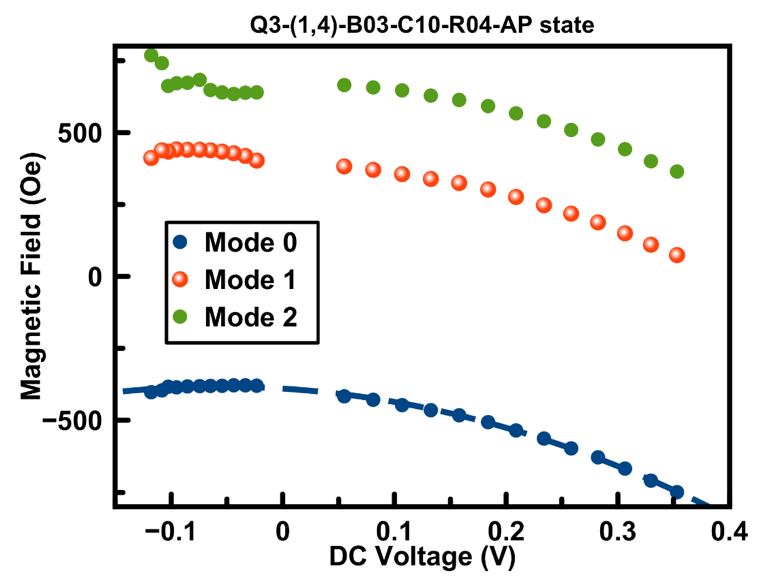
\includegraphics[width=75mm]{fig/2018/C10DC-FH}}
\subfigure{\label{fig:C10DCLW}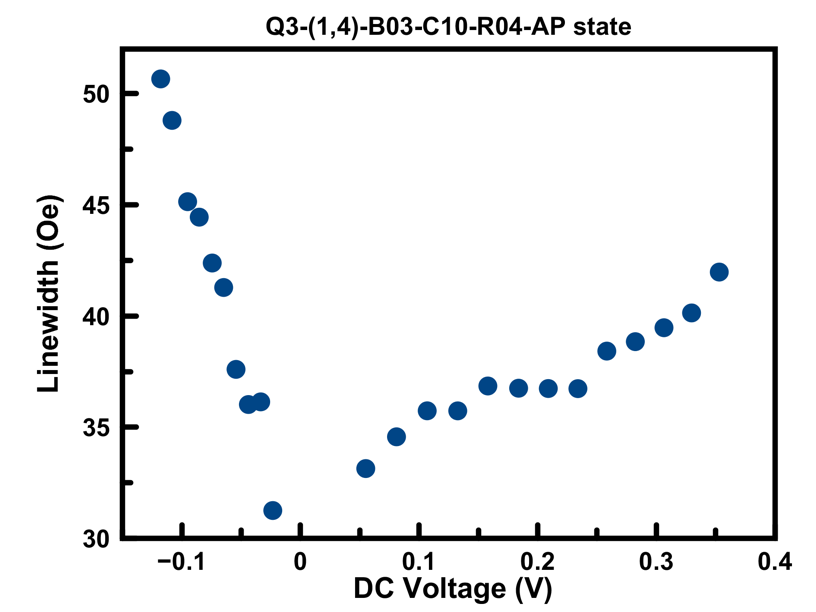
\includegraphics[width=75mm]{fig/2018/C10DC-LW}}
\caption{}
\end{figure}



\newpage

\section{Summary of Circular Devices}



\begin{figure}[!ht]
  \centering
  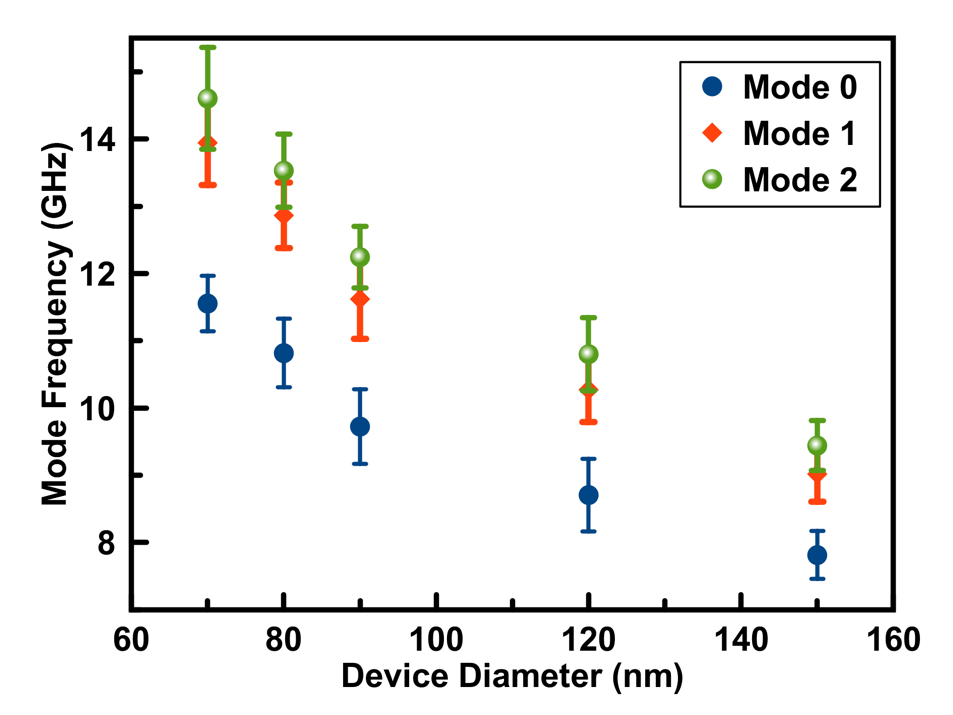
\includegraphics[width=0.6\textwidth]{fig/2018/ModevsSize}
   \caption{Mode vs Size}
  \label{fig:ModeVsSize}
\end{figure}



The effective demagnetization factor is
\begin{equation}\label{eq:Nz}
	\centering
	N_z \approx 1- \frac{1}{\pi d} [2 \ln(4 \frac{d}{t} ) -1 ]
\end{equation}

where the d is the device diameter and t is the free layer thickness. Eq.\ref{eq:Nz}

The total perpendicular anisotropy $H_ku$ can be written as 

\begin{equation}\label{eq:Hk}
	\centering
	H_k = H_{ku} + 2 \pi (1 - 3 N_z) M_s
\end{equation}

Assuming the free layer thickness 1.6 nm, the fitted result $M_s$ 1820 emu/cm^3 and $H_{ku}$ 24 KOe.



\begin{figure}[!ht]
\centering
\subfigure{\label{fig:GapvsSize}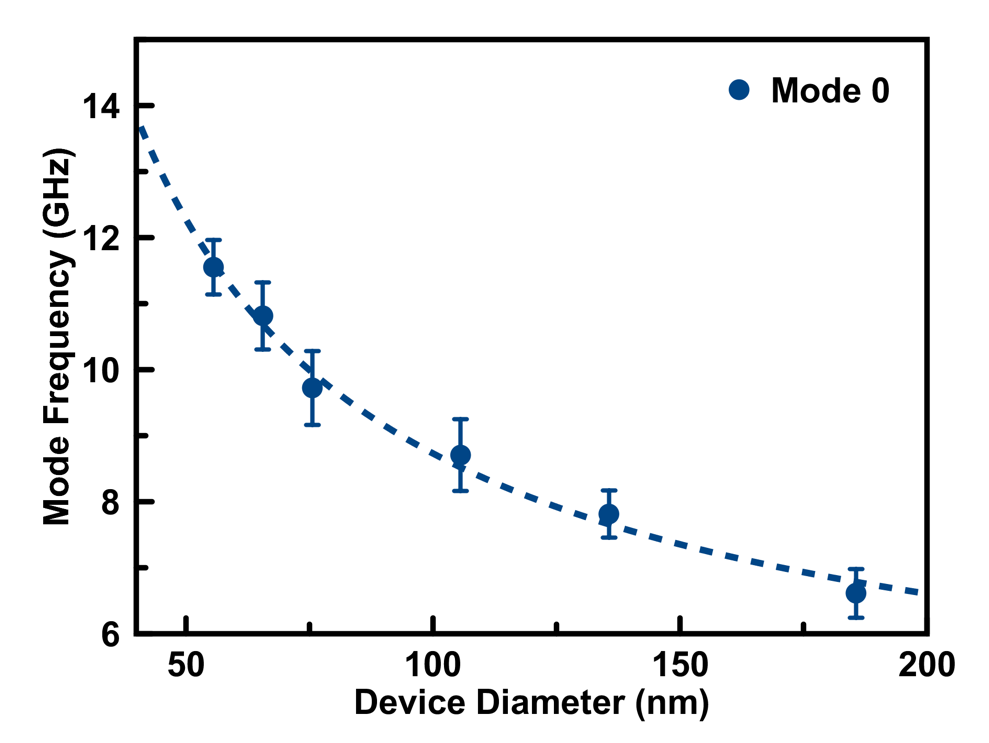
\includegraphics[width=75mm]{fig/2018/GapvsSize}}
\subfigure{\label{fig:LinearFit}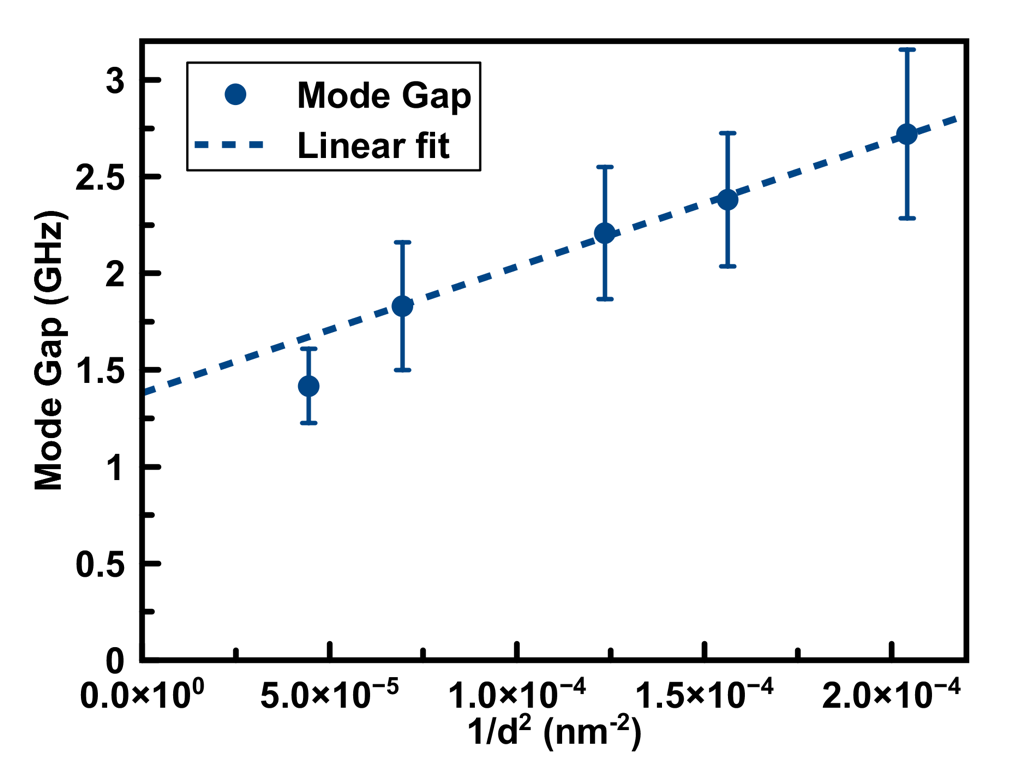
\includegraphics[width=75mm]{fig/2018/LinearFit}}
\caption{}
\end{figure}





